%!TEX root = ../template.tex
%%%%%%%%%%%%%%%%%%%%%%%%%%%%%%%%%%%%%%%%%%%%%%%%%%%%%%%%%%%%%%%%%%%%
%% chapter3.tex
%% NOVA thesis document file
%%
%% Chapter with the Model (what I did)
%% topics:
%% Solution
%% Intro, what I did
%% what I did in the platform, (Zoom)
%%Architecture
%% uml, digrama de sequencia, arvora de decisão, solução do paper, %%tabela com o  formato da mensagens
%%%%%%%%%%%%%%%%%%%%%%%%%%%%%%%%%%%%%%%%%%%%%%%%%%%%%%%%%%%%%%%%%%%%

\chapter{Adaptive Geolocation}
\label{cha:Adaptive_Geolocation}

In today's solutions for locating people with dementia, there is the lack of a system capable of locating a person and at the same time being able to dynamically choose the best location, thus saving battery power. 
This chapter describes the intended model for this dissertation.
It is proposed as a module that is part of the Carelink platform.


\section{Overview}
\label{sec:overview}

The above-mentioned platform is represented in~\ref{fig:Platform_Archictecture}, and it was designed to be safe, extendable and perform well in the future. To achieve this, the micro-services approach was adopted, where logically distinct elements of application code are developed and deployed separately. These services communicate with each other using a combination of REST and messages. This enables services to be continually improved and new services to be implemented whenever needed. 

\begin{figure}[htbp]
  \centering
  
    {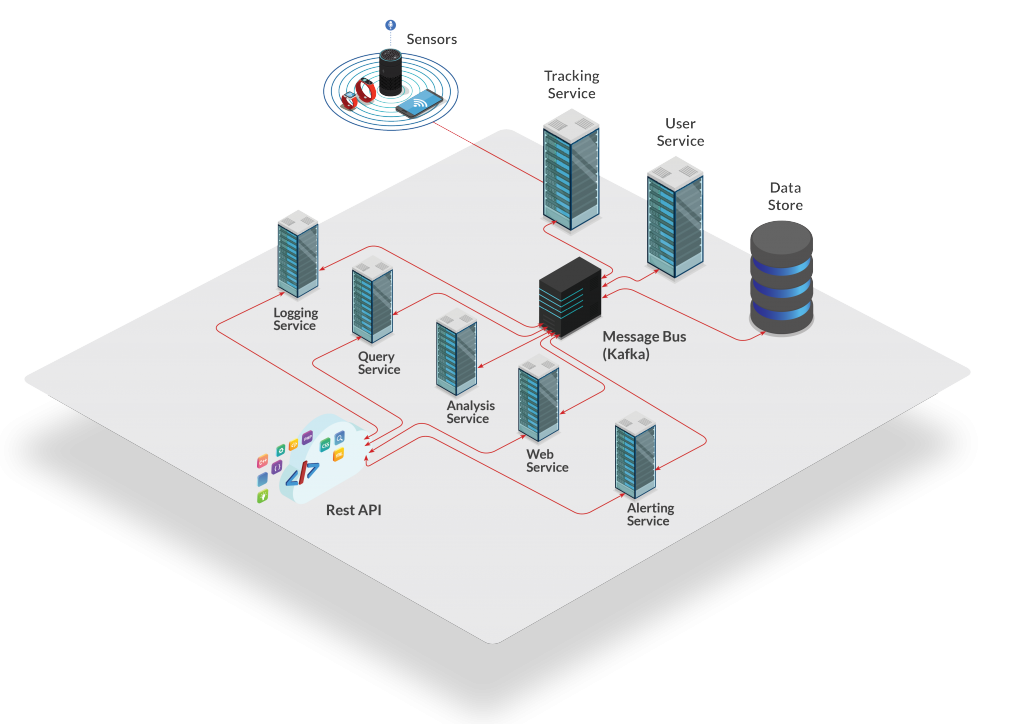
\includegraphics[width=1\linewidth]{Chapters/Figures/Carelink-Diagrams-1024x724.png}}%
 
  \caption{Carelink Platform Architecture~\cite{carelink}}
  \label{fig:Platform_Archictecture}
\end{figure}
One of the services present in the platform is the tracking service. This micro-service acts as a consumer of the output, from the proposed model. 
The model acts as a bridge between the physical world, composed by the hardware devices, and the respective sensors, and the virtual world represented by the Carelink platform.

The location of people with dementia, demands a resilient and fast system, capable of offering real-time data, structured in such a way that is easy to present and visualize, so the next module is capable without much effort to present in a graphical away the information, allowing the user fast access to this one.
Since the situation when a person with dementia, has an episode of wandering, is highly stressful, for the caregivers or person in charge, is imperative that the system is able to provide an accurate location without being too complex, because this system is intended to track devices that are connected to persons, not to assets or animals, is one main requirement to have high availability.\newline\newline


The model must be prepared to receive, as well as, interpret messages from different devices and transmission types (LoRa, NB-IoT). In order to achieve this must be device agnostic, the way to solve this issue is using a naming convention for the protocol of communication (MQTT). 
Following the same ideology of the platform, it must also be divided into small modules, to be easily scalable, and allow updates without large changes to the core implementation, being more future proof. This approach also benefits the model with a more easy and manageable way of implement security, monitoring and redundancy.

As the information may arrive at different rates, or even in the worst-case fail, the model functionalities, work in modules that are independent and they can work isolated, as well as, in parallel. To solve this problem inside of one particular module, was used smart gate queuing and load balancing techniques.

To conclude was intended that the model, alongside with is integrated system, were capable of performing a location, taking into account the remaining battery of the device, and in the end create a profile-based decision system, in charge of dynamically choose the best location, providing this way the adaptive geolocation capability.





\newpage
\section{Adaptive Geolocation Solver}
The Adaptive Geolocation Solver is the model which is part of the system, that compose the solution. The main objective for this model is receiving the messages from the devices, and return the best possible location.


\label{sec:adaptive_geolocation_solver}
\subsection{Model Schematic}
The next figure~\ref{fig:Model_Schematic} introduces the model schematic for the adaptive geolocation solver.
This model is composed by different modules each of one with a different function. Following this image will be the explanation of each module, as well as, the main functions present inside of each module.

\begin{figure}[htbp]
  \centering
  
    {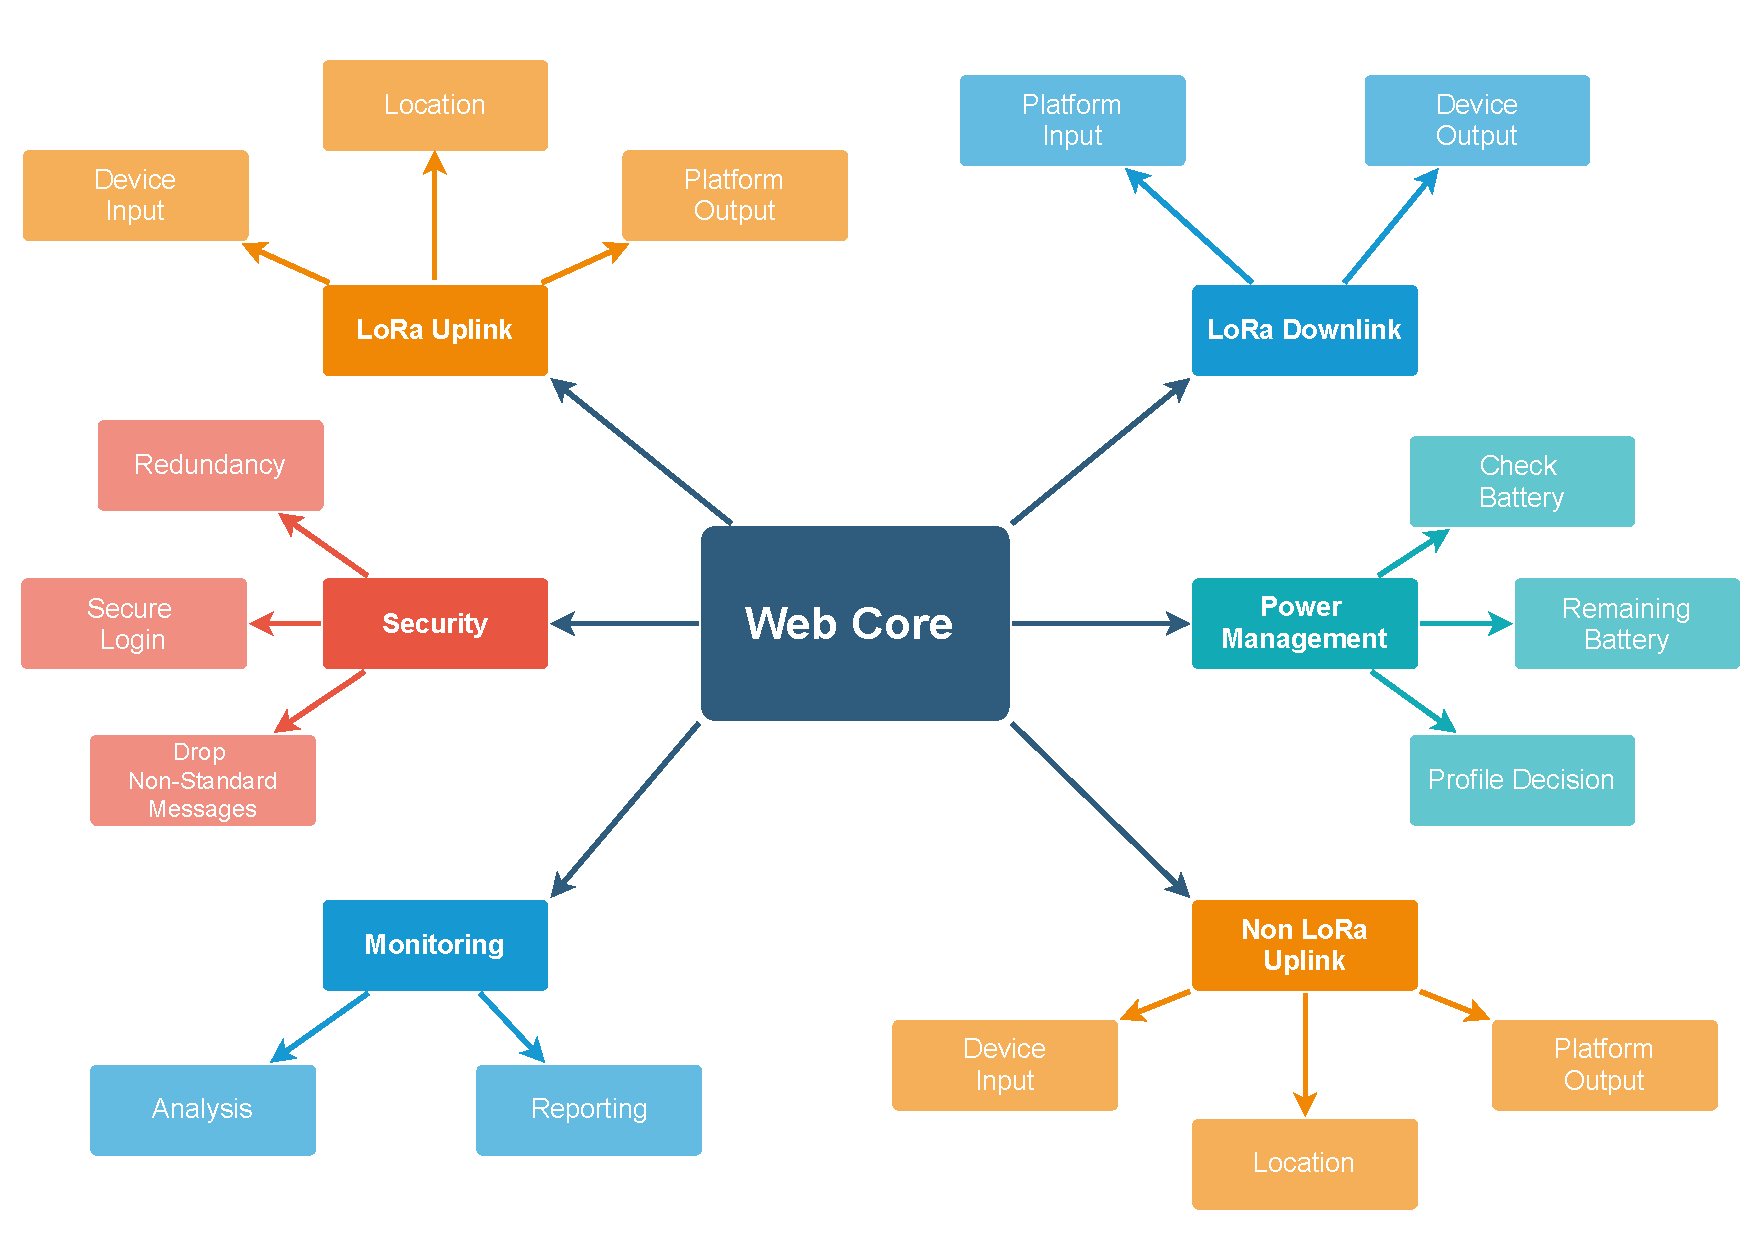
\includegraphics[height= 4in,width=0.92\linewidth]{Chapters/Figures/model_schematic3.pdf}}%
 
  \caption{Mind Map for Model Schematic}
  \label{fig:Model_Schematic}
\end{figure}



\begin{itemize}
\item \textbf{Web Core} \\
This is the core module where all the others are built on top. The main characteristics of this module will be discussed in more detail in the next chapter~\ref{cha:Implementation}, but essentially it is a web server capable of running JavaScript functions.
\end{itemize}

\begin{itemize}
\label{susec:Lora_to_Platform}
   \item \textbf{LoRa Uplink} \\
   This first module is responsible for, the incoming messages. when the previous transmission method was LoRa. This module is responsible for the  next functions.
   \begin{itemize}
     \item Device Input: \\
      The messages received from LoRa transmission and are stored in a smart gate  queue.
   \end{itemize}
   \begin{itemize}
     \item Location: \\
      After the message is ready to be processed, is filtered to look up for the location information. The best location is joined to the original message.
   \end{itemize}
   \begin{itemize}
     \item Platform Output: \\
      In the end, the right device is selected and  the combined message is sent to the Platform.
   \end{itemize}
\end{itemize}


\begin{itemize}
   \item \textbf{LoRa Downlink} \\
   The Carelink platform can communicate directly with devices, through MQTT, but this is not possible directly using LoRa (as explained in the next chapter~\ref{cha:Implementation}), so this module acts as a middle layer for the communication. 
   \begin{itemize}
     \item Platform Input:\\ 
     The different MQTT topics are subscribed, and the message is received. Then is converted to JSON, and encrypted to Base64.
   \end{itemize}
   \begin{itemize}
     \item Device Output: \\
     After the message passes to Base64, and the correct topic is selected. This function selects the right device and sends the message.
   \end{itemize}
\end{itemize}


\begin{itemize}
   \item \textbf{Power Management}\\
   This module is in charge of all the power management capabilities of the model, and it is composed by the following functions. 
   \begin{itemize}
     \item Check Battery: \\This function is responsible for analysing the received message, verify the battery level, and the communications that are currently in use. 
   \end{itemize}
   \begin{itemize}
     \item Remaining Battery: \\Where the battery level is converted into the remaining battery duration.
   \end{itemize}
   \begin{itemize}
     \item Profile Decision: \\Using the previous information, decide which profile to use.
   \end{itemize}
\end{itemize}


\begin{itemize}
   \item \textbf{Non LoRa Uplink} \\
    This module shares the same functions as the "LoRa Uplink", however, is designed to be more communication agnostic, and therefore serve more devices. 
\end{itemize}


\begin{itemize}
   \item \textbf{Security} \\
The "Security"  module is responsible for the correct operation of the model. This module consists of the following functions.
   \begin{itemize}
     \item Redundancy: \\
      This function is achieved, through the "LoRa to Platform" and "Other to Platform", by having more than one path to transmit the message to the platform.
      Inside both, there is also a redundancy location mechanism.
      The last redundancy feature is the fact of the "Web Core" is running in a docker container. 
   \end{itemize}
   \begin{itemize}
     \item Secure Login:  \\
      The access to the "Web Core" is done using a login with username and password, but the password is not stored, only the hash.
   \end{itemize}
   \begin{itemize}
     \item Drop Non-Standard Messages: \\
      All the incoming messages that are Non-standard are filtered and drop, securing the model and make it more efficient.
   \end{itemize}
\end{itemize}

\begin{itemize}
   \item \textbf{Monitoring} \\
   Using the following functions, and with the ability to connect with the other modules, is capable of ensuring the normal operation for the model.
   \begin{itemize}
     \item Analysis:\\
     This function is mainly done in the "LoRa to Platform" and "Other to Platform" modules, where the number of messages flowing, is registered in different points.
   \end{itemize}
   \begin{itemize}
     \item Reporting: \\
     Making use of the previous knowledge of "Analysis", this function generates a daily e-mail report, and at an abnormal situation, where the non-processed messages achieve a defined threshold, this functions sends an SMS message.
   \end{itemize}
\end{itemize}

\begin{itemize}
   \item \textbf{Development}\\
   This last module exists but is not represented in the schematic, since it is not used in a production environment. The development module aims, to provide a sandbox, where the following features can be tested, alongside with the other modules that are in a production environment, but without being in production.
   \begin{itemize}
     \item Debugging:  \\This  function is used in case something goes wrong. It is possible to replicate,  to find the error.
   \end{itemize}
   \begin{itemize}
     \item Updates Testing: \\When the error is found, it is possible to develop and test an update. After some iterations, the update is finished and ready for production. 
   \end{itemize}
   \begin{itemize}
     \item Map visualization: \\ In order to have a place for visualization of the data, in a real world map, to get an idea of what is going to be shown next, in the platform, and for easy interpretation of the data, was created this function.
   \end{itemize}
\end{itemize}









\newpage
\subsection{Stages \& Operation}
\label{susec:Stages_Operation}

The aim of the presented work is the development and implementation of this model. This model intends to define what technologies to use, and how the geolocation data from different sources should be processed, so that it can later be used for knowing the actual position of the patient wearing the device.

In order to develop the solution described, it was defined a model to characterize and formalize the different types of solutions called stages. Later an implementation following the model defined occurred creating the so-called profile based decision system.

The next diagram~\ref{fig:Stages}, represents the three different functional stages, called: “hierarchical”, “advanced” and “smart”. The Venn diagram is then followed by the explanation of each stage.

\begin{figure}[htbp]
  \centering
  
   % {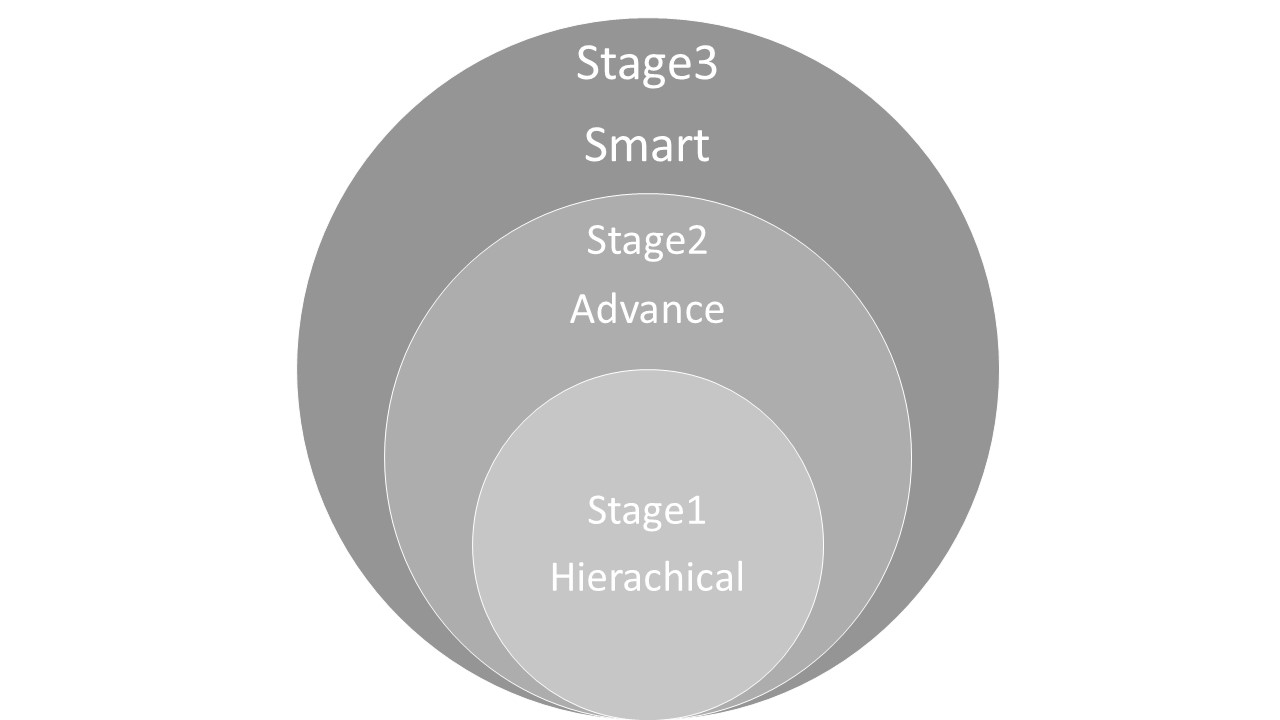
\includegraphics[height=2.4in,width=0.8\linewidth]{Chapters/Figures/Stages.jpg}}%
   {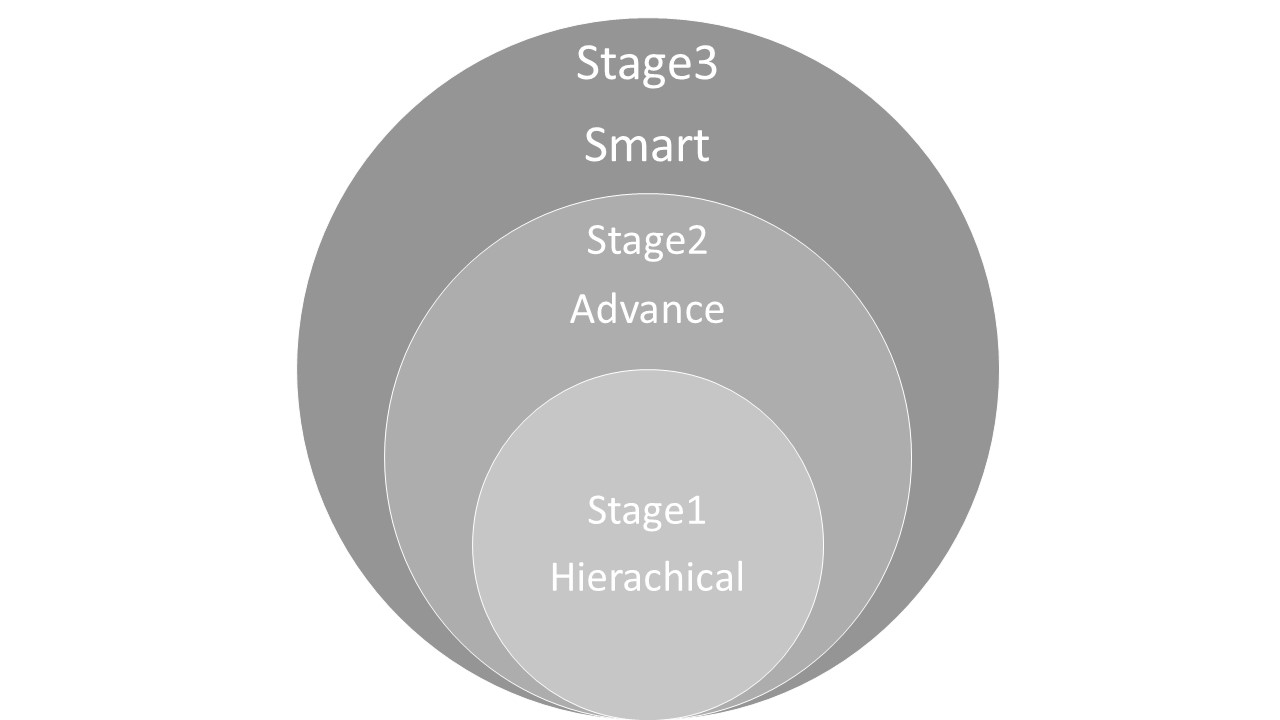
\includegraphics[width=0.55\linewidth]{Chapters/Figures/Stages.jpg}}
 
  \caption{Model Stages}
  \label{fig:Stages}
\end{figure}
%maior

\begin{itemize}
\item \textbf{Stage 1} - Hierarchical 
\end{itemize}


The first stage called hierarchical, in which the best location is decided using the approximate accuracy values of each method. Taking into account the documentation, and the tests performed, the accuracy defined was $GNSS > WiFi > LoRa$.

\begin{figure}[htbp]
  \centering
  
    {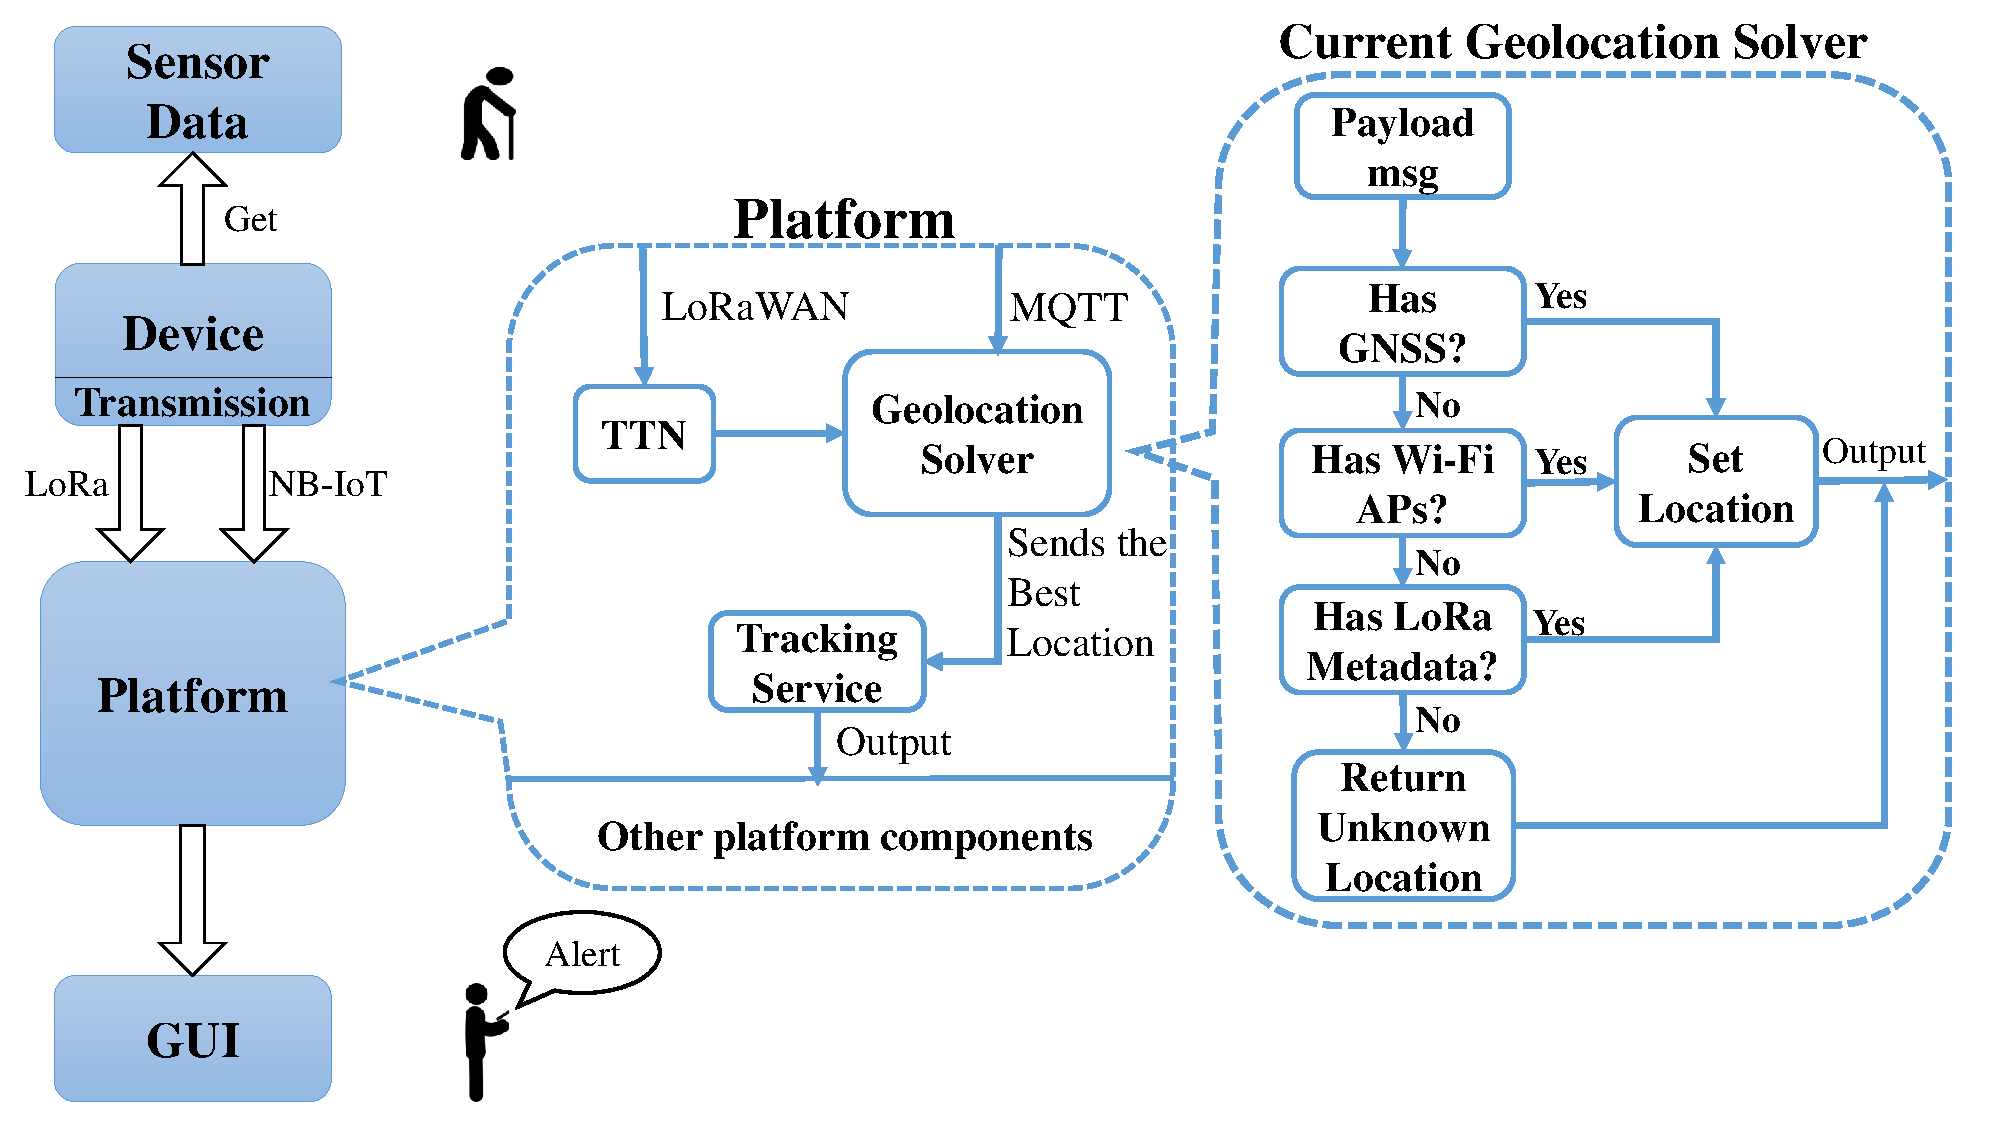
\includegraphics[width=0.7\linewidth]{Chapters/Figures/modelarch.pdf}}%
  \caption{System and Model Architecture - Hierarchical version~\ref{app:paper}}
  \label{fig:Model_overview}
\end{figure}
Based on the proposed model the author started to
develop the profile-based decision system. In this initial phase, it only includes the "hierarchical" functional stage. Its architecture is represented in Figure~\ref{fig:Model_overview}. 
In the right dotted square from this figure, is the workflow behind the "Geolocation Solver" block, that is  where the model is working, and its operation is described in the following.
First as described at~\ref{susec:Lora_to_Platform} on page~\pageref{susec:Lora_to_Platform}, an input message from the device is received containing a JSON, there exists an object with the status of the device. This status message has the following fields:
\begin{figure}[htbp]
  \centering
    \scalebox{0.9}{
    {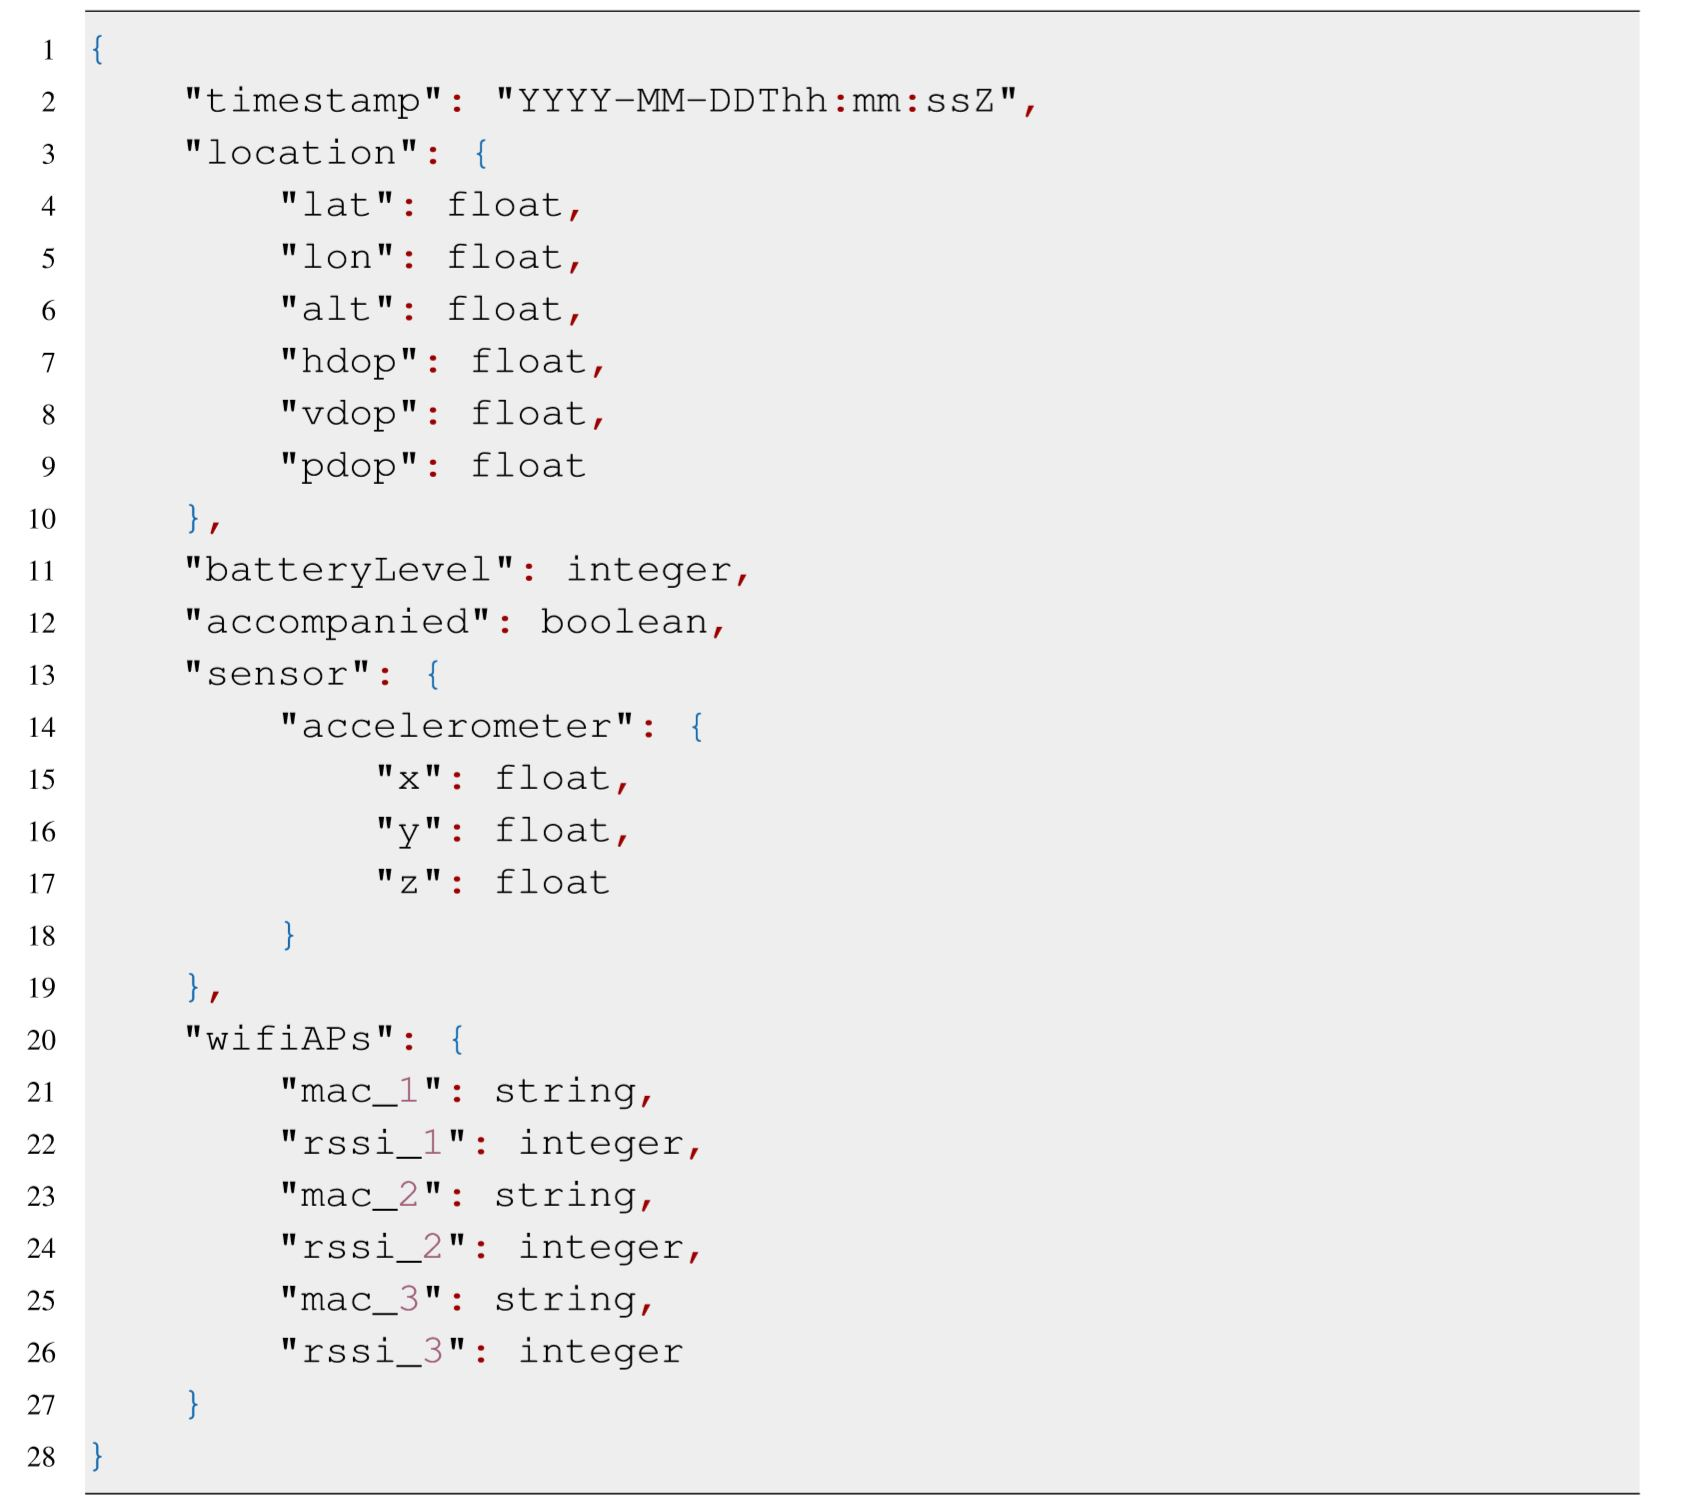
\includegraphics[width=\linewidth]{Chapters/Figures/JSONStatus.jpg}}%
    }
  \caption{JSON Status Payload}
  \label{fig:JSON_Status}
\end{figure}
%%%%%%%%%%%%% 

In the first block "Has GNSS?", the location field of~\ref{fig:JSON_Status} is analyzed. There are two options, for the coordinates or they are valid or not. If the coordinates provided are valid, and to accomplish this the latitude and longitude fields, need to be simultaneous different from zero. If the information is valid, the location is set, and then forwarded to the Tracking service in Carelink platform. The unused information for the other methods is dropped.\newline On the other hand, the received messages where these fields are zero, are considered invalid because they came with the default value from the device. In the situation where the coordinates provided, arrive with a type different from float, will also be considered invalid, since a transmission error occurred.


\newpage
%%%%%%%%%%%%%%%%%%%%%%%%%%%% Stage 1 Wifi %%%%%%%%%%%%%%%%%%

In case the location field is empty or the coordinates are considered not valid, the following block is the “Has Wi-Fi APs?”. In this, the "wifiAPs"  field from the above-mentioned JSON object is analysed. If it is different from null, this payload is used to perform the assisted location, based on the Wi-Fi data. This data will then be sent to three different API,  using a load balancer, which is  based in the sequential Round Robin. This is done to obtain the best information for the location, and at the same time use fewer APIs calls, and prevent the APIs from refuse the requests. The three used APIs in this work were, Google Geolocation API, Here Position API and OpenCelliD Cellular Geolocation API. This load balancer uses the following equation:

\begin{equation} \label{eq:loadbalancer}
    h(x) = \begin{cases}
        HO & \text{, }x \in {3n+1}\\
        HG & \text{, }x \in {3n+2}
        \hspace{5mm} n \in \mathbb{N}_{0} \\
        OG & \text{, }x \in {3n+3}
        \end{cases} 
\end{equation}
In the previous equation~\ref{eq:loadbalancer}:
\begin{itemize}
	\item {$H$} - Here 
	\item {$O$} - OpenCelliD
	\item {$G$} - Google

\end{itemize} 
After receiving the response, the information is compared between the two used APIS, in order to guarantee redundancy, as well as, the best accuracy possible. And then it is combined in the JSON Status, and the unused fields are discarded. In the end, this JSON is also forwarded to the platform.

%%%%%%%%%%%%%%%%%%%%%%%%%% Stage1 LoRa %%%%%%%%%%%%%%

If the communication method in use was LoRa, then the LoRa metadata will also be used to apply different geolocation algorithms, such as multilateration, based on received signal strength or the time  difference of arrival. The result is the approximated device location. For this last method work, with reliability, a minimum of three gateways in range is needed. In the scenario where all of the three previous blocks, failed to  return a valid location, it is returned location unknown.


\begin{figure}[htbp]
  \centering
    \scalebox{0.35}{
    {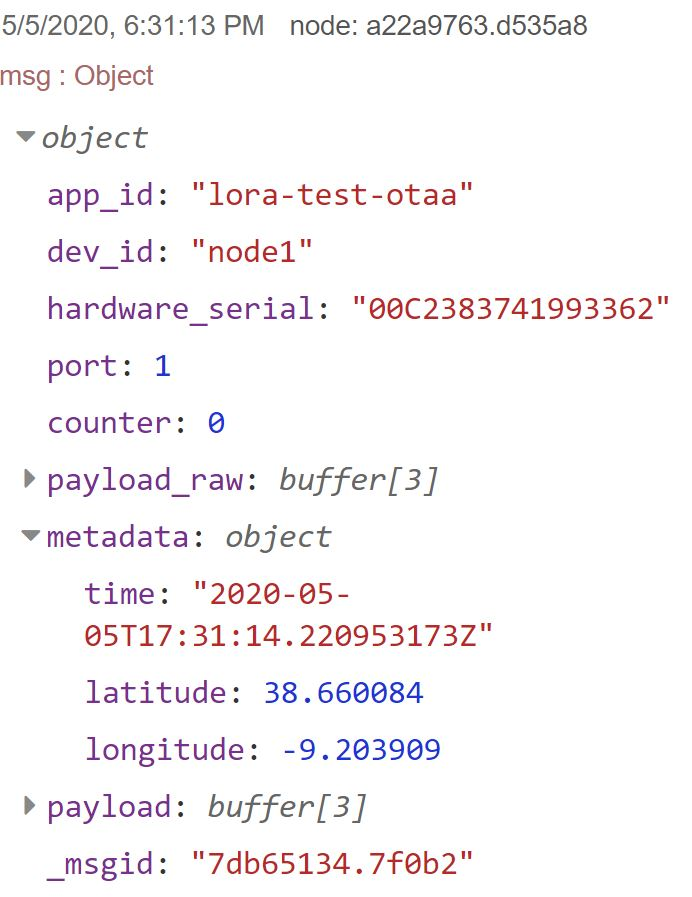
\includegraphics[width=\linewidth]{Chapters/Figures/LoRaMetadata.JPG}}%
    }
  \caption{LoRa Location Metadata}
  \label{fig:LoRa_Metadata}
\end{figure}


%%%%%%%%%%%%%%%%%%%%%%%%%%%%%%% Stage1 end %%%%%%%%%%%%%%%%%%%%
\newpage

\begin{itemize}
\item \textbf{Stage 2} - Advance
\end{itemize}


The second stage formalises the location decision
function based on two characteristics at the same time: the
battery level of the device and the location accuracy for the
chosen technology, thus being more “advanced”. 
This stage also adds another location method, the location through beacons BLE, that can be used indoors. This beacons have a short-range, and are used in the situation where GNSS is not working, and there is no WiFi available, for example, the house of a person with dementia, in a rural place. 
Alongside with the addition of this location method, there is also an addition of WiFi, for transmitting the data, in the device side. This is not model related, since the model is agnostic to the transmission method, but it was a step taken in this stage.

In this stage for assuring the high availability needed for this work, the geolocation function should be capable of
knowing the remaining battery. In case the person is in a dangerous situation, or in an area that was previously assigned as unsafe, this stage does the balance between the optimal location and the more power efficient location.
As represented in the following figure~\ref{fig:Stage2_State_MAchine}, where the different numbers $(1, 2, 3, 4)$ represent the different levels of Geolocation accuracy, and battery saving. Using path $1$ exists more location sources, so it has higher accuracy, but also require more battery. 

\begin{figure}[htbp]
  \centering
    \scalebox{0.29}{
    {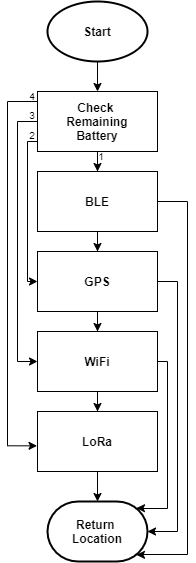
\includegraphics[width=\linewidth]{Chapters/Figures/Stage2State.pdf}}%
    }
  \caption{Stage 2 State Machine }
  \label{fig:Stage2_State_MAchine}
\end{figure}

\newpage
\begin{itemize}
\item \textbf{Stage 3} - Smart 
\end{itemize}

In the last stage, a more advanced location function is formalised. Its decision capability for choosing the technologies to use, are based in the surrounding environment. For example, if a patient is not showing any activity by a long period of time, it is night time and he/she is in a safe place, as the home it can be deduced that the person is sleeping, and therefore the sampling time for the location can be reduced, thus saving battery.
Another example is by combining additional
sensor data, such as  an accelerometer that can detect if the~\gls{PwD} has fallen, the priority can be given to the method with the best accuracy, because of this dangerous situation.

This stage introduces the addition of SigFox and Pymesh, for transmitting the data, in the device side. SigFox has a daily limit for the Uplink messages, and a maximum size too small to transmit a full message, therefore, is only used in the worst-case scenario. The Pymesh uses LoRa but only the LoRa Modulation to create a mesh network between the devices, this is the method of the last resource when all the others failed.

To conclude, this last stage combines a set of different
factors to categorize and do a profile-based decision.

\begin{table}[htbp]
\centering
\scalebox{0.65}{
\begin{tabular}{cc|c|c|c|c|c|c|}
\cline{3-8}
 &  & \multicolumn{2}{c|}{HOME} & \multicolumn{2}{c|}{\begin{tabular}[c]{@{}c@{}}Outside\\ Safe Zone\end{tabular}} & \multicolumn{2}{c|}{\begin{tabular}[c]{@{}c@{}}Outside\\ Unsafe Zone\end{tabular}} \\ \hline
\multicolumn{2}{|c|}{\begin{tabular}[c]{@{}c@{}}PwD\\ STATUS\end{tabular}} & Accompanied & Alone & \multicolumn{1}{l|}{Accompanied} & Alone & Accompanied & Alone \\ \hline
\multicolumn{1}{|c|}{\cellcolor[HTML]{FFFFC7}} & \begin{tabular}[c]{@{}c@{}}Day\\ Time\end{tabular} & \begin{tabular}[c]{@{}c@{}}BLE\\ WiFi\\ Sensors 20 min\end{tabular} & \begin{tabular}[c]{@{}c@{}}BLE\\ WiFi\\ Sensors 15 min\end{tabular} & \begin{tabular}[c]{@{}c@{}}LoRa\\ NB-IoT\\ GNSS 30 min\\ Sensors 30 min\end{tabular} & \begin{tabular}[c]{@{}c@{}}LoRa\\ NB-IoT\\ GNSS 15 min\\ Sensors 30 min\end{tabular} & \begin{tabular}[c]{@{}c@{}}LoRa\\ NB-IoT\\ GNSS 15 min\\ Sensors 15 min\end{tabular} & \begin{tabular}[c]{@{}c@{}}LoRa\\ NB-IoT\\ GNSS 10 min\\ Sensors 10 min\end{tabular} \\ \cline{3-8} 
\multicolumn{1}{|c|}{\cellcolor[HTML]{FFFFC7}Normal} &  &  &  &  &  &  &  \\
\multicolumn{1}{|c|}{\cellcolor[HTML]{FFFFC7}} & \begin{tabular}[c]{@{}c@{}}Night\\ Time\end{tabular} & \begin{tabular}[c]{@{}c@{}}BLE\\ WiFi\\ Sensors 1 hour\end{tabular} & \begin{tabular}[c]{@{}c@{}}BLE\\ WiFi\\ Sensors 30 min\end{tabular} & \begin{tabular}[c]{@{}c@{}}LoRa\\ NB-IoT\\ GNSS 1 hour\\ Sensors 30 min\end{tabular} & \begin{tabular}[c]{@{}c@{}}LoRa\\ NB-IoT\\ GNSS 30 min\\ Sensors 30 min\end{tabular} & \begin{tabular}[c]{@{}c@{}}LoRa\\ NB-IoT\\ GNSS 30 min\\ Sensors 30 min\end{tabular} & \begin{tabular}[c]{@{}c@{}}LoRa\\ NB-IoT\\ GNSS 5 min\\ Sensors 5 min\end{tabular} \\ \hline
\multicolumn{1}{|c|}{\cellcolor[HTML]{FFCE93}} & \begin{tabular}[c]{@{}c@{}}Day\\ Time\end{tabular} & \begin{tabular}[c]{@{}c@{}}BLE\\ WiFi\\ Sensors 15 min\end{tabular} & \begin{tabular}[c]{@{}c@{}}BLE\\ WiFi\\ NB-IoT\\ Sensors 5 min\end{tabular} & \begin{tabular}[c]{@{}c@{}}LoRa\\ NB-IoT\\ GNSS 15 min\\ Sensors 15 min\end{tabular} & \begin{tabular}[c]{@{}c@{}}LoRa\\ NB-IoT\\ GNSS 10 min\\ Sensors 10 min\end{tabular} & \begin{tabular}[c]{@{}c@{}}LoRa\\ WiFi\\ NB-IoT\\ GNSS 10 min\\ Sensors 5 min\end{tabular} & \begin{tabular}[c]{@{}c@{}}LoRa\\ WiFi\\ NB-IoT\\ GNSS 5 min\\ Sensors 5 min\end{tabular} \\ \cline{3-8} 
\multicolumn{1}{|c|}{\cellcolor[HTML]{FFCE93}Warning} &  &  &  &  &  &  &  \\
\multicolumn{1}{|c|}{\cellcolor[HTML]{FFCE93}} & \begin{tabular}[c]{@{}c@{}}Night\\ Time\end{tabular} & \begin{tabular}[c]{@{}c@{}}BLE\\ WiFi\\ Sensors 30 min\end{tabular} & \begin{tabular}[c]{@{}c@{}}BLE\\ WiFi\\ NB-IoT\\ Sensors 10 min\end{tabular} & \begin{tabular}[c]{@{}c@{}}LoRa\\ NB-IoT\\ GNSS 15 min\\ Sensors 15 min\end{tabular} & \begin{tabular}[c]{@{}c@{}}LoRa\\ NB-IoT\\ GNSS 10 min\\ Sensors 10 min\end{tabular} & \begin{tabular}[c]{@{}c@{}}LoRa\\ WiFi\\ NB-IoT\\ GNSS 5 min\\ Sensors 5 min\end{tabular} & \begin{tabular}[c]{@{}c@{}}LoRa\\ WiFi\\ NB-IoT\\ GNSS 2 min\\ Sensors 2 min\end{tabular} \\ \hline
\multicolumn{1}{|c|}{\cellcolor[HTML]{FD6864}} & \begin{tabular}[c]{@{}c@{}}Day\\ Time\end{tabular} & \begin{tabular}[c]{@{}c@{}}BLE\\ WiFi\\ Sensors 10 min\end{tabular} & \begin{tabular}[c]{@{}c@{}}BLE\\ LoRa\\ WiFi\\ NB-IoT\\ Sensors 1 min\end{tabular} & \begin{tabular}[c]{@{}c@{}}LoRa\\ WiFi\\ NB-IoT\\ GNSS 10 min\\ Sensors 5 min\end{tabular} & \begin{tabular}[c]{@{}c@{}}LoRa\\ WiFi\\ NB-IoT\\ GNSS 5 min\\ Sensors 1 min\end{tabular} & \begin{tabular}[c]{@{}c@{}}BLE\\ LoRa\\ Mesh\\ WiFi\\ SigFox\\ NB-IoT\\ GNSS 5 min\\ Sensors 1 min\end{tabular} & \begin{tabular}[c]{@{}c@{}}BLE\\ LoRa\\ Mesh\\ WiFi\\ SigFox\\ NB-IoT\\ GNSS 1 min\\ Sensors 1 min\end{tabular} \\ \cline{3-8} 
\multicolumn{1}{|c|}{\cellcolor[HTML]{FD6864}Danger} &  &  &  &  &  &  &  \\
\multicolumn{1}{|c|}{\cellcolor[HTML]{FD6864}} & \begin{tabular}[c]{@{}c@{}}Night\\ Time\end{tabular} & \begin{tabular}[c]{@{}c@{}}BLE\\ LoRa\\ WiFi\\ NB-IoT\\ Sensors 5 min\end{tabular} & \begin{tabular}[c]{@{}c@{}}BLE\\ LoRa\\ WiFi\\ NB-IoT\\ Sensors 1 min\end{tabular} & \begin{tabular}[c]{@{}c@{}}LoRa\\ WiFi\\ NB-IoT\\ GNSS 10 min\\ Sensors 5 min\end{tabular} & \begin{tabular}[c]{@{}c@{}}LoRa\\ WiFi\\ NB-IoT\\ GNSS 5 min\\ Sensors 1 min\end{tabular} & \begin{tabular}[c]{@{}c@{}}BLE\\ LoRa\\ Mesh\\ WiFi\\ SigFox\\ NB-IoT\\ GNSS 5 min\\ Sensors 1 min\end{tabular} & \begin{tabular}[c]{@{}c@{}}BLE\\ LoRa\\ Mesh\\ WiFi\\ SigFox\\ NB-IoT\\ GNSS 1 min\\ Sensors 30 sec\end{tabular} \\ \hline
\end{tabular}
}
\caption{Operation Mode Profiles}
\label{tab:Profiles}
\end{table}
 
 
 
 
 
 
 
 
 
 
 
 
 
 
 

 
 
 
 
 
 
 
\newpage
\section{Summary}
\label{summary}
In summary, the system that was is illustrated in Figure~\ref{fig:Model_overview}, to which the proposed model will be contributing, as one of the building blocks. 

The first step in the proposed system is to collect sensor data from the~\gls{PwD} wearing the device. Afterwards, a specific transmission method is selected, of which the options may vary from LoRa to NB-IoT.
The second step, already inside of the platform, is to combine the previous information in the purposed model called Adaptive Geolocation Solver, in order to get the best location possible, this model had different stages of development has described in~\nameref{susec:Stages_Operation}, as well as, is constituted by 6 has it is possible to observe at~\nameref{sec:adaptive_geolocation_solver}. 

The Carelink platform, alongside with the model, is responsible for managing the devices, and ensure the high availability needed, in order to always know the location of the patient, especially when this one is having an episode of wandering and its lost. 
The final geolocation information is then passed on to the corresponding micro-service, in this case, the tracking service, and then the final step is sending the response from the tracking service to the GUI.
Once in the GUI the user responsible for the patient can be alerted,  when a geofencing alert is raised, with the information that the person has crossed to an unsafe area.

To conclude the next~\acrshort{SWOT} analysis of the model summarizes the different aspects of this work. From the data in the orange corner is possible to observe that one drawback of this work is the maximum number of processed messages. In the grey square is presented to the reader, the threats of this work being the first threat the dependency from 3rd party providers, for the locations done through API. The last threat is the PwD Acceptance, this threat consists of convincing the PwD and the respective caregiver that the proposed solution could benefit both.


\begin{figure}[htbp]
\centering
%%% SWOT matrix
\colorlet{helpful}{lime!70}
\colorlet{harmful}{red!30}
\colorlet{internal}{yellow!20}
\colorlet{external}{cyan!30}
\colorlet{S}{helpful!50!internal}
\colorlet{W}{harmful!50!internal}
\colorlet{O}{helpful!50!external}
\colorlet{T}{harmful!50!external}

\newcommand{\texta}{Helpful\par}
\newcommand{\textb}{Harmful\par}
\newcommand{\textcn}{Internal origin\par}
\newcommand{\textdn}{External origin\par}

\newcommand{\back}[1]{\fontsize{60}{70}\selectfont #1}




\begin{tikzpicture}[
    any/.style={minimum width=4cm,minimum height=4cm,%
                 text width=2.7cm,align=center,outer sep=0pt},
    header/.style={any,minimum height=1cm,fill=black!10},
    leftcol/.style={header,rotate=90},
    mycolor/.style={fill=#1, text=#1!60!black}
]

  
\matrix (SWOT) [matrix of nodes,nodes={any,anchor=center},%
                column sep=-\pgflinewidth,%
                row sep=-\pgflinewidth,%
                row 1/.style={nodes=header},%
                column 1/.style={nodes=leftcol},
                inner sep=0pt]
{
          &|[fill=helpful]| {\texta} & |[fill=harmful]| {\textb} \\
|[fill=internal]| {\textcn} & |[mycolor=S]| \back{S} & |[mycolor=W]| \back{W} \\
|[fill=external]| {\textdn} & |[mycolor=O]| \back{O} & |[mycolor=T]| \back{T} \\
};

\node[any, anchor=center] at (SWOT-2-2) {High \\Availability \\ Adaptive Location};
\node[any, anchor=center] at (SWOT-2-3) { Maximum number of processed messages};
\node[any, anchor=center] at (SWOT-3-2) {Scalabale\\ Communication agnostic};
\node[any, anchor=center] at (SWOT-3-3) {3rd party\\Providers\\PwD \\Acceptance};
 

\end{tikzpicture}
 
  \caption{\gls{SWOT} Matrix}
  \label{fig:swot}
\end{figure}








 
 

 
 



